% !TEX encoding = UTF-8 Unicode
\chapter{Das Konzept des Revenue Managements}\label{KapitelDP}
\markboth{3 Revenue Management}{}
\setcounter{footnote}{4}  %um durchgehende Fußnotennummerierung zu haben, hier die Anzahl der bisherigen Fußnoten eintragen


\section{Herkunft des Revenue Managements}
Zur Entscheidungsunterstützung bei der Annahme von Kundenaufträgen wird in der aktuellen Forschung vermehrt auf das Konzept des Revenue Managements zurückgegriffen.\footnote{Vgl. \cite{klein2001revenue}, S. 246.} Da eine kurzfristige Anpassung der mittelfristig bereitgestellten Kapazitäten einer Dienstleistungsproduktion an eine unsichere und schwankende Nachfrage nicht möglich ist, wird mit dem Konzept eine effizientere Auslastung der bestehenden Kapazitäten ermöglicht.\footnote{Vgl. \cite{ing2005revenue}, S. 124.}

Der Begriff \textit{Revenue Management} wird im deutschsprachigen Raum meist mit \textit{Ertrags}\-\textit{management} oder \textit{Erlösmanagement} übersetzt.\footnote{Vgl. z. B. \cite{zehle1991yield}, S. 486} Yield Management wird als Synonym benutzt.\footnote{Vgl. z. B. \cite{kolisch2006revenue}, S. 319} Dabei greift der Begriff \textit{Yield} zu kurz, da damit in der Luftverkehrsbranche der Erlös je Passagier und geflogener Meile bezeichnet wird.\footnote{Vgl. z. B. \cite{weatherford1998tutorial}, S. 69} Der Term \textit{Revenue Management} hat sich jedoch gegenüber Yield Management durchgesetzt, da der Yield (Durchschnittsertrag) sich theoretisch nur durch einen Passagier maximieren lässt und somit die Maximierung als Zielsetzung nicht sinnvoll ist.\footnote{Vgl. \cite{Klein:2008aa}, S. 6; \cite{ing2005revenue}, S. 124-125.} Erste Ansätze des RM sind in der Praxis entwickelt. Durch die Deregulierung des amerikanischen Luftverkehrsmarktes im Jahr 1978 mussten die traditionellen Fluggesellschaften ihre Wettbewerbsfähigkeit gegenüber Billiganbietern erhöhen und entwickelten das frühe RM.\footnote{Vgl. \cite{Petrick:2009aa}, S. 1-3}

\cite{kimms2005revenue} versuchen durch eine umfangreiche Diskussion einige Erklärungsansätze aufzuzeigen (Warum? Wovon?). Das RM hat vor allem aus dem älteren, englischsprachigen Bereich einen engen Bezug zu konkreten Anwendungsgebieten. Die Autoren zeigen auf, dass viele Autoren versuchen das komplexe Konzept des Revenue Managements in einer kurzen Erklärung zu überführen. Dieses läuft letztlich darauf hinaus, dass diese Autoren einige situative Merkmale und Instrumente des Managements vermischen, gleichzeitig aber versuchen, die Zielsetzung festzulegen und das Anwendungsgebiet auf bestimmte Branchen zu beschränken. %\cite{kimms2005revenue} weisen darauf hin, dass eine differenzierte Betrachtung des Konzepts notwenig ist: Einerseits im Hinblick auf die Anwendungsvoraussetzungen und andererseits im Hinblick auf die Instrumente des Revenue Managements, damit verdeutlicht dargestellt wird, in welchen Branchen das RM Potentiale liefert. In den nachfolgenden zwei Kapiteln wird dieser Empfehlung gefolgt.

Weiter wird in der Literatur der Begriff des RM unterschiedlich definiert. \cite{friege1996yield} bezeichnet das RM als \textit{Preis-Mengen-Steuerung}, \cite{daudel1992yield} als \textit{Preis-Kapazitäts-Steuerung} und \cite{talluri2004theory} verstehen es als das gesamtes \textit{Management der Nachfrage}. Die beiden ersteren Definitionen können als Synonym für eines der Instrumente des RM stehen und daher finden diese für das gesamte Konzept keine weitere Verwendung.\footnote{Vgl. z. B. \cite{Petrick:2009aa}} Nachfolgend wird die Definition von \citeauthor{klein2001revenue} (2001, S. 248) aufgegriffen:

\begin{quote}
\glqq Revenue Management umfasst eine Reihe von quantitativen Methoden zur Entscheidung über Annahme oder Ablehnung unsicherer, zeitlich verteilt eintreffender Nachfrage unterschiedlicher Wertigkeit. Dabei wird das Ziel verfolgt, die in einem begrenzten Zeitraum verfügbare, unflexibel Kapazität möglichst effizient zu nutzen.\grqq
\end{quote}

\cite{Petrick:2009aa} definiert das RM als Ziel einer Unternehmung die Gesamterlöse zu maximieren, die sich aufgrund der speziellen Anwendungsgebiete ergeben. Damit definiert \cite{Petrick:2009aa} das RM als Zusammenfassung aller Interaktionen eines Unternehmens, die mit dem Markt, also der Absatz- oder Nachfrageseite, zusammenhängen. Im Kern lassen sich drei wichtige Perspektiven für eine Definition des Revenue Managements nach \cite{Petrick:2009aa}, \cite{stuhlmann2000kapazitatsgestaltung},  \cite{corsten1999yield} übernehmen:
\begin{enumerate}
	\item Ziel ist es die Gesamterlöse unter möglichst optimaler Auslastung der vorhandenen Kapazitäten zu maximieren.
	\item Durch eine aktive Preispolitik wird das reine Kapazitäts- oder Auslastungsmanagement unterstützt.
	\item Für die erfolgreiche Implementierung des Revenue Managements ist eine umfangreiche Informationsbasis notwendig. Es muss u. a. eine möglichst gute Prognose über die zukünftige Nachfrage und Preisbereitschaft der Kunden vorhanden sein.
\end{enumerate}

\cite{kimms2005revenue} weisen darauf hin, dass eine differenzierte Betrachtung des Konzepts notwenig ist: Einerseits im Hinblick auf die \textbf{Anwendungsvoraussetzungen} und andererseits im Hinblick auf die \textbf{Instrumente des Revenue Managements}, damit verdeutlicht dargestellt ist, in welchen Branchen das RM Potentiale liefert. Dabei sollten branchenspezifische Besonderheiten, neben den zahlreichen Ähnlichkeiten Berücksichtigung finden, sowie das begrenzte Kapazitätenkontingent, damit die Potentiale des RM zur Maximierung der Gesamterlöse in den Dienstleistungsbranchen erfolgen kann.\footnote{Vgl. z. B. \cite{Martens:2009aa}, S. 11-24} In dem nachfolgenden Kapitel wird dieser Empfehlung gefolgt und die Anwendungsvoraussetzungen sowie Instrumente des RM vorgestellt.

\section{Anwendungsvoraussetzungen und Instrumente des Revenue Managements}

\cite{Petrick:2009aa} weist da\-rauf hin, dass anhand von speziellen Anwendungsvoraussetzungen geprüft wird, ob das RM für die jeweilige Situation des Unternehmens (oder die gesamte Branche) zur Maximierung des Gesamterlöses beiträgt. \cite{kimes1989yield} definiert die in der Literatur häufigsten Anwendungsvoraussetzungen:\footnote{Vgl. u. a. \cite{friege1996yield}, S. 616-622, und \cite{weatherford1992taxonomy}, 831-832.}
\begin{itemize}
	\item \glqq weitgehend fixe\grqq\;Kapazitäten
	\item \glqq Verderblichkeit\grqq\;bzw. \glqq Nichtlagerfähigkeit\grqq\;der Kapazitäten und der Leistung
	\item Möglichkeit zur Vorausbuchung von Leistungen
	\item stochastisch, schwankende Nachfrage
	\item hohe Fixkosten für die Bereitstellung der gesamten Kapazitäten bei vergleichsweise geringen variablen Kosten für Produktion einer Leistungseinheit
	\item Möglichkeit zur Marktsegmentierung und im Ergebnis dessen zur segmentorientierten Preisdifferenzierung
\end{itemize}
\vspace{0.2cm}
Aufgrund der Anwendungsvoraussetzungen des RM kann das Konzept auch auf die Auftragsfertigung bzw. MRO-Prozesse übertragen werden.\footnote{Vgl. \cite{hintsches2010revenue}, S.176-178; \cite{kimes1989yield}, S. 349-351.} Bei der Auftragsfertigung wird ein bestimmter Buchungszeitraum betrachtet, in dem weitestgehend von fixen Kapazitäten der Ressourcen ausgegangen werden kann. Durch Ablauf des Buchungshorizonts verfällt die Kapazität, da es sich hauptsächlich um erneuerbaren Kapazitäten handelt (Arbeitskraft, Maschinenkapazität, usw.). Anders formuliert, die Ressourcen werden zur nächsten Leistungserstellung erneuert. Dabei beschreibt $t$ einen Zeitpunkt des Buchungshorizonts. Die Gesamtlänge des Buchungshorizonts entspricht $T$ und verläuft rückwärts bis zur Leistungserstellung des betrachteten Buchungshorizonts. Da der Buchungshorizont mit genau einer Leistungserstellung gekoppelt ist, können diese mit einem Parameter $i$ beschrieben werden. Mit der Leistungserstellung werden die verbuchten Kapazitäten aus dem Buchungshorizont durch die Auftragsproduktion beansprucht. Mit dem Start der Leistungserstellung erfolgt ebenfalls die Vorausbuchungszeit für die nachfolgende Leistungserstellung $i+1$. Bei der Leistungserstellung $i+1$ sind die Kapazitäten der Ressourcen regeneriert. Abbildung \ref{B0} zeigt den Zusammenhang von Buchungshorizont, Leistungserstellung und abnehmenden Ressourcenkapazität.

% Grafik noch falsch!!!
\begin{figure}[h!]
  \begin{center}
    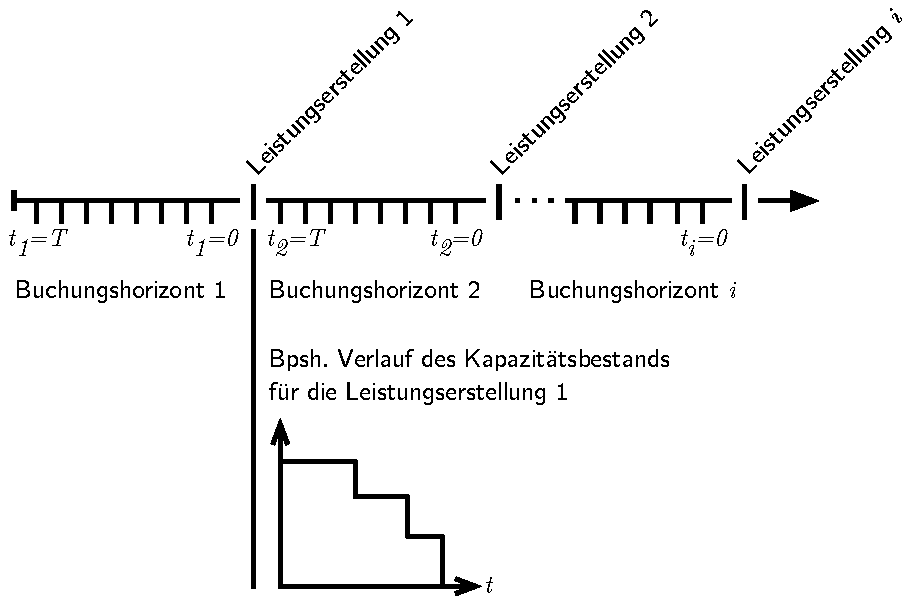
\includegraphics[width=140mm]{Bilder/Kapaverbrauch.pdf}
    \caption{Grafische Darstellung des Buchungshorizonts bei der Auftragsfertigung}  \label{B0}
    {\footnotesize \textbf{In Anlehnung an:} ???.} 
  \end{center}
\end{figure}


??? \cite{Klein:2008aa} setzen sich mit den Anwendungsvoraussetzungen von mehreren Autoren auseinander. Sie konnten Gemeinsamkeiten innerhalb der Definitionen der Autoren finden, aber zeigten auch die Unterschiede und die Kritiken auf. In ihrer Arbeit übernehmen sie die Anwendungsvoraussetzung von \cite{corsten1998yield}: "Marktseitige Anpassungserfordernis steht unternehmesseitigig unzureichendes Flexibilitätspotential hinsichtlich der Kapazität -- bezogen auf Mittel- oder Zeitaufwand -- gegenüber". Zugleich weisen sie jedoch darauf hin, dass zum Verständnis eines komplexen und interdisziplinären Ansatzes auch die Definitionen anderer Autoren im Hinblick auf das Verständnis der Anwendungsvoraussetzungen beitragen. ???

Auf Grundlage der von \cite{friege1996yield} beschriebenen Anwendungsvoraussetzungen hat \cite{Petrick:2009aa} drei Instrumente des RM bestimmt. Die Instrumente benötigen als Grundlage \textit{Daten der Prognose}, damit sie zur Anwendung kommen.\footnote{Die Prognose zählt laut \cite{Petrick:2009aa} nicht als eigenständiges Instrument des RM.} Zu den Instrumenten zählen die \textbf{segmentorientierte Preisdifferenzierung}, die \textbf{Kapazitäten\-steuerung} und die \textbf{Über\-buchungssteuerung}. Es lassen sich unterschiedliche Ab\-hängigkeit\-en der Instrumente untereinander ermitteln.\footnote{Als Beispiel baut die Kapazitätensteu\-erung auf den Ergebnissen der Preisdifferenzierung auf und die Überbuchungssteuerung kann selten ohne Kapazitätensteuerung gelöst werden.}

Erklärung segmentorientierte Preisdifferenzierung, Kapazitätssteuerung, Überbuchungssteuerung?

\section{Mathematische Modellformulierung des Revenue Managements}\label{Grundmodell}
Im Folgenden wird das dynamisch, stochastische Grundmodell des RM nach \citeauthor{talluri2004revenue} (2004, S. 18-19) beschrieben. Ein Dienstleistungsnetzwerk eines Anbieters benötigt jeweils zur Erstellung der Dienstleistungen ein bestimmtes Kontingent an Ressourcen aus einer Menge an Ressourcen $\mathcal{H} = \{1,...,l \}$. Der Index $h$ beschreibt dabei eine jeweilige Ressource und der Index $l$ die gesamte Anzahl an möglichen Ressourcen. Die jeweilige Kapazität einer Ressource $h \in \mathcal{H}$ ist durch den Parameter $c_{h}$ beschrieben und die gesamten Kapazitäten der Ressourcen ist als Vektor $\textbf{c}=(c_{1},...,c_{h},...,c_{l})$ formuliert. Eine Anfrage nach einem Produkt (Dienstleistung) in dem Netzwerk ist durch den Parameter $j$ aus der Menge an möglichen Produktanfragen $\mathcal{J} = \{1,...,n \}$ %für die Menge der Ressourcen $\mathcal{H}$
beschrieben. Die gesamte Anzahl an Produktanfragen ist durch den Parameter $n$ definiert. Sobald eine Produktanfrage $j\in \mathcal{J}$ akzeptiert und somit abgesetzt ist, fällt für den Absatz der Ertrag $r_{j}$ an. Der jeweilige Verbrauch einer Ressource $h$ durch Annahme einer Anfrage nach einem Produkt $j$ ist anhand des Parameters $a_{hj}$ beschrieben. Durch Vektorschreibweise kann der Ressourcenverbrauch für eine Anfrage nach einem Produkt $j$ als Vektor $\textbf{a}_{j}=(a_{1j},...,a_{hj},...,a_{lj})$ formuliert werden. Der Buchungshorizont entspricht $T$ Perioden und kann jeweils in einzelne Perioden $t=1,...,T$ aufgeteilt werden. Dabei muss Beachtung finden, dass der Buchungshorizont $T$ gegenläufig verläuft. Die Wahrscheinlichkeit der Nachfrage eines Produkts $j$ in der Periode $t$ entspricht $p_{j}(t)$ und die Wahrscheinlichkeit, dass keine Nachfrage in der Periode $t$ eintrifft, entspricht $p_{0}(t)$. Es gilt $\sum_{j\in \mathcal{J}}p_{j}(t)+p_{0}(t)=1$ und somit kann $p_{0}(t)$ durch den Term $p_{0}(t)=1-\sum_{j\in \mathcal{J}}p_{j}(t)$ für die Periode $t$ ermittelt werden.\footnote{Vgl. \citeauthor{talluri2004revenue}, S. 18} Die noch erwartete Nachfrage $D_{jt}$ für ein bestimmtes Produkt $j$ für eine beliebige Periode $t$ lässt sich durch $\sum_{\tau=1}^{t}p_{j}(\tau)$ aggregieren. 


Mit den vorangegangenen Parametern kann der maximal erwartete Ertragswert $V(\textbf{c},t)$ für eine Periode $t$ bei einer noch vorhandenen Ressourcenkapazität $\textbf{c}$ als Bellman-Gleichung formuliert werden (\textbf{DP-op}):\footnote{???}
\begin{equation}\label{DP}
V(\textbf{c},t)=\sum_{j\in\mathcal{J}}p_{j}(t)\max[ V(\textbf{c},t-1),\; r_{j}+V(\textbf{c}-\textbf{a}_{j},t-1)]+p_{0}(t)V(\textbf{c},t-1)
\end{equation}


Es handelt sich hier um die Modellformulierung der Dynamischen Programmierung (DP) im Netzwerk RM. Das Konzept der DP wurde von \citeauthor{bellman1954theory} entwickelt und dient der Ermittlung der optimalen Politik in Bezug auf den aktuellen Zustand eines Systems.\footnote{Vgl. \cite{bellman1954theory}, S. 4-5} Dabei bildet jeder Erwartungswert $V(\textbf{c},t)$ mit der Ressourcenkapazität $\textbf{c}$ zum Zeitpunkt $t$ einen Systemzustand des Netzwerks ab. Eine derartige Formulierung eines Optimierungsproblems wird oft als sogenannte \textit{Bellman'sche Funktionsgleichung oder Bellman-Gleichung} bezeichnet.\footnote{???}

Die Gleichung weist die Grenzbedingungen
\begin{equation}\label{GB1}
V(\textbf{c},0)=0 \text{ wenn } \textbf{c}\ge0 \text{ sowie }
\end{equation}
\begin{equation}\label{GB2}
V(\textbf{c},t)=-\infty \text{ wenn } c_{j}<0 \;\forall j\in\mathcal{J}
\end{equation}
auf, da eine jeweilig verbleibende Kapazität nach Bereitstellung des Produkts wertlos und eine negative Ressourcenkapazität nicht möglich ist. 

Die Gleichung \eqref{DP} lässt sich umformen, indem die Entscheidungen über die Annahme und Ablehnung einer Produktanfrage separiert wird. Da $\sum_{j\in \mathcal{J}}p_{j}(t)+p_{0}(t)=1$ gilt, kann die Gleichung weiter vereinfacht werden:\footnote{Vgl. \cite{Spengler:2007aa}, S. 161.}
\begin{equation}\label{DP2}
\begin{alignat*}{2}
V(\textbf{c},t)=\;& \sum_{j\in\mathcal{J}}p_{j}(t) V(\textbf{c},t-1)+ \sum_{j\in\mathcal{J}}p_{j}(t) \max[0,r_{j}-V(\textbf{c},t-1)\\
&+V(\textbf{c}-\textbf{a}_{j},t-1)]+p_{0}(t)V(\textbf{c},t-1)\\
=\;& V(\textbf{c},t-1) + \sum_{j\in\mathcal{J}}p_{j}(t) \max[0,\\
&  r_{j}-V(\textbf{c},t-1)+V(\textbf{c}-\textbf{a}_{j},t-1)]
\end{alignat*}
\end{equation}

Eine eintreffende Anfrage nach einem Produkt $j$ ist demnach dann akzeptiert, wenn der Ertrag $r_{j}$ größer gleich der Differenz des Erwartungswertes des Ertrags unter der Prämisse der Annahme der Produktanfrage und des Erwartungswertes des Ertrag unter der Prämisse der Ablehnung der Produktanfrage ist:
\begin{equation}\label{r}
r_{j} \ge V(\textbf{c},t-1)-V(\textbf{c}-\textbf{a}_{j},t-1)
\end{equation}

Dabei kann der rechte Term \eqref{r} als Opportunitätskosten (OK) der Auftragsannahme angesehen werden:
\begin{equation}\label{OC}
OC_{j} = V(\textbf{c},t-1)-V(\textbf{c}-\textbf{a}_{j},t-1)
\end{equation}

Somit erfolgt die Akzeptanz einer Anfrage nach einem Produkt $j\in\mathcal{J}$ ausschließlich nur dann, sofern die OK des Ressourcenverbrauchs niedriger als der Ertrag ist. Der maximal mögliche Erwartungswert unter Beachtung des Kapazität $\textbf{c}$ zum Zeitpunkt $t$ ist damit der Erwartungswert unter der Prämisse der Ablehnung der Anfrage zum nächsten Zeitpunkt $t-1$ inkl. der Summe der Erträge abzgl. der OK durch Annahme der möglichen Anfragen über aller Produkte $j\in\mathcal{J}$ und lässt sich mathematisch wie folgt definieren:
\begin{equation}\label{DPoc}
V(\textbf{c},t)=V(\textbf{c},t-1) + \sum_{j\in\mathcal{J}}p_{j}(t) \max[0,r_{j}-OC_{j}]
\end{equation}

%Die optimale Politik des Netzwerks zum Zeitpunkt $t$ ist damit die Annahme der Anfrage nach Produkt $j$ mit dem höchsten Ertrag $r_{j}$ abzüglich der anfallenden $OC_{j}$:

%begin{equation}\label{OP}
%OP_{\textbf{c}, t}:= \{ \; j\; | \max_{j\in\mathcal{J}} [r_{j}-OC_{j}] \} 
%\end{equation}

Zur Veranschaulichung des Netzwerk RM wird ein Netzwerk mit zwei Produkten $j\in\mathcal{J}$ und zwei Ressourcen $h\in\mathcal{H}$ betrachtet. Die Ressource $h=1$ hat eine Kapazität von $c_{1}=2$ und die Ressource $h=2$ hat eine Kapazität von $c_{2}=1$. Zur Ausführung des Produkt $j=1$ wird die Ressource $h=1$ mit einer Einheit benötigt und zur Ausführung des Produkt $j=2$ wird wiederum eine Einheit der Ressource $h=2$ gebraucht. Damit gilt $a_{11}=1$ und $a_{22}=1$. Durch Annahme einer Anfrage nach Produkt $j=1$ wird der Ertrag $r_{1}=100$ und durch Annahme von Produkt $j=2$ eine Ertrag von Ertrag $r_{2}=200$ generiert. Der Buchungshorizont entspricht $T=4$. Die Wahrscheinlichkeiten des Eintreffens eine Anfrage nach Produkt $j=1$ über die Buchungsperioden $t\in T$ lässt sich als Vektor $p_{1}(t)=(0.5, 0.5, 0.5, 0.5)$ beschreiben. Analog lassen sich die Wahrscheinlichkeiten für das Eintreffen der Produktanfragen $j=2$ als Vektor $p_{2}(t)=(0.1, 0.1, 0.1, 0.1)$ definieren. Die Gegenwahrscheinlichkeiten, dass keine Anfragen eintreffen, lassen sich mit $p_{0}(t)=1-\sum_{j\in \mathcal{J}}p_{j}(t)$ berechnen und bilden den Vektor $p_{0}(t)=(0.4, 0.4, 0.4, 0.4)$. Durch Vereinfachung der Gleichung \eqref{DP} zur Gleichung \eqref{DP2} werden die Gegenwahrscheinlichkeiten $p_{0}(t)$ nicht mehr benötigt und im weiteren Verlauf der Arbeit nicht mehr berücksichtigt.

Die Parameter lassen sich damit abschließend wie folgt definieren:
\begin{center}
$j = \{1, 2\}, \; h = \{1, 2\}, \; r_{1} = 100, \; r_{2} = 200, \; \text{Startperiode } t=4$,
\end{center}
\[
    \textbf{c}=\begin{pmatrix} 2 \\ 1 \end{pmatrix}, \;
    \textbf{a}_1=\begin{pmatrix} 1 \\ 0 \end{pmatrix}, \;
     \textbf{a}_2=\begin{pmatrix} 0 \\ 1 \end{pmatrix}, \;
     p_{1}(t)=\begin{pmatrix} 0.5\\ 0.5\\ 0.5\\ 0.5  \end{pmatrix}, \;
     p_{2}(t)=\begin{pmatrix} 0.1\\ 0.1\\ 0.1\\ 0.1  \end{pmatrix}
  \]

Die mathematische Modellformulierung des stochastisch, dynamisches Programms aus Gleichung \eqref{DP2} lässt sich als Graph darstellen, der die einzelnen Systemzustände für die DP aufzeigt.\footnote{Vgl. \cite{demiguel2006multistage}, S. 8-13.} Der Erwartungswert $V(\textbf{c},t)$ ist abhängig vom Erwartungswert $V(\textbf{c},t-1)$ und vom Erwartungswert $V(\textbf{c}-\textbf{a}_{j},t-1)$. Der Erwartungswert $V(\textbf{c},t-1)$ ist wiederum abhängig vom Erwartungswert $V(\textbf{c},t-2)$ und vom Erwartungswert $V(\textbf{c}-\textbf{a}_{j},t-2)$, usw. Abbildung \ref{B0} zeigt die erste rekursive Folge für die Gleichung \eqref{DP2} als gerichteten Graphen auf und im nachfolgenden wird auf die Notation eingegangen.
\begin{figure}[h!]
  \begin{center}
    \includegraphics[width=80mm]{Bilder/Beispiel0.pdf}
    \caption{Beispielhafte Darstellung einer rekursive Folge eines Netzwerk RM}  \label{B0}
  \end{center}
\end{figure}

Ein Knoten repräsentiert einen Systemzustand des Netzwerks mit den vorhandenen Kapazitäten $\textbf{c}$ zum Zeitpunkt $t$. Bei dem Systemzustand handelt es sich um ein Teilproblem des Modells. Bei der Benennung eines solchen Knotens wird eine Zahlenfolge verwendet, bei dem die ersten Einträge die Ressourcenkapazität $\textbf{c}$ in Länge der Ressourcen $h$ entsprechen und der letzte Eintrag den Zeitpunkt $t$ aufzeigt. Bspw. zeigt der Startknoten des Beispiels die Zahlenfolge $[2\;1\;4]$, da das Netzwerk noch die volle Ressourcenkapazität $\textbf{c}=(2,1)$ aufweist und sich im Zeitpunkt $t=4$ befindet. Von diesem Systemzustand können jetzt nachfolgende Systemzustände abhängig der Produktanfragen erreicht werden. In diesem Netzwerk gibt es zwei Produkte $j$ und durch betrachten der Gleichung \eqref{DP2} wird klar, dass drei Optionen zum Erreichen des nachfolgenden Systemzustands zum Zeitpunkt $t-1=3$ möglich sind. Diese Optionen bilden die Kanten des Graphen. Es kann keine Anfrage nach einem Produkt $j$ eintreffend, dann wird der nachfolgende Systemzustand $[2\;1\;3]$ erreicht. Alternativ können Anfragen nach Produkt $j=1$ oder $j=2$ eintreffen und dementsprechend müssen die vorhanden Kapazitäten $\textbf{c}$ um den Ressourcenverbrauch $a_{11}=1$ bzw. $a_{22}=1$ reduziert werden. Daraus folgt, dass der Systemzustand $[1\;1\;3]$ bzw. $[2\;0\;3]$ im Netzwerk erreicht werden kann. Die optimale Politik eines solchen Graphen wird abgebildet durch die Kanten. Sofern der Übergang des Systemzustands durch Annahme der jeweiligen Anfrage $j$ gegen die Bedingung \eqref{OC} verstößt, wird die Kante des Graphen als gestrichelter Pfeil dargestellt. Ein Übergang über die Kante zum nächsten Systemzustand wäre theoretisch möglich, aber entspricht nicht der optimalen Politik.

Aufbauen auf dieser rekursiven Logik wird ein gerichteter und gewichteter Multigraph aufgebaut. Er zeigt alle möglichen Systemzustände des Netzwerks. Die Rekursion wird abgebrochen, sofern ein Systemzustand aufgrund der Grenzbedingungen aus den Gleichungen \eqref{GB1} oder \eqref{GB2} nicht möglich ist. Abbildung \ref{B1} zeigt die möglichen Systemzustände für das eingeführte Beispiel.
\begin{figure}[h!]
  \begin{center}
    \includegraphics[width=150mm]{Bilder/Beispiel1.pdf}
    \caption{Darstellung der Systemzustände des beispielhaften Netzwerk RM}  \label{B1}
  \end{center}
\end{figure}

Anhand dieses Graphen mit den möglichen Systemzuständen aus der Abbildung \ref{B1} wird ersichtlich, welche Erwartungswerte (Teilprobleme) für das Entscheidungsproblem der Auftragsannahme durch Rückwärtsinduktion gelöst werden müssen.\footnote{Vgl. ???, S. ???.} Dafür wird im ersten Schritt die Grenzbedingung aus Gleichung \eqref{GB1} betrachtet. Alle Systemzustände zum Zeitpunkt $t=0$ nehmen den Erwartungswert $V(\textbf{c}, t=0)=0$ an. Mit dieser Bedingung lassen sich die zeitlich zuvorkommenden Systemzustände mit $t=1$ berechnen. Es wird die Gleichung \eqref{DP2} angewendet, wobei beachtet werden muss, dass nicht für alle Systemzustände mit $t=1$ alle Produktanfragen möglich sind. Dies folgt aus der Grenzbedingung aus Gleichung \eqref{GB2}. Zur Veranschaulichung wird der Erwartungswert des Systemzustands $[1\;0\;1]$ mittels der Gleichung \eqref{DP2} berechnet.
\begin{alignat*}{2}
V(1,0,1)=\;&V(1,0,0)+p_{1}(1)\max[r_{1}-V(1,0,0)+V(0,0,0),0]\\
&+p_{2}(1)\max[r_{2}-V(1,0,0)+V(0,-1,0),0]\\
=\;&0+0,5\cdot\max[100-0+0,0]+0,1\cdot\max[200-0+(-\infty),0]\\
=\;&0+0,5\cdot 100+0,1\cdot0\\
=\;&50\\
\end{alignat*}
Nach dieser Vorgehensweise der Rückwärtsinduktion erfolgt die Ermittlung alle Erwartungswerte der möglichen Systemzustände. Tabelle \ref{Tab1} zeigt für alle möglichen Systemzustände $[c_1\;c_2\;t]$ den Erwartungswerten (ExpValue) und die optimale Politik. Die optimale Politik ist in den letzten zwei Spalten der Tabelle \ref{Tab1} jeweils für die zwei möglichen Anfragen $j\in\mathcal{J}$ aufgeführt. Sofern eine Anfrage nach dem Produkt $j$ eintrifft, zeigt die Tabelle mit dem Wert $\glqq 1\grqq$, dass die Anfrage unter den Bedingungen der vorhandenen Kapazitäten $\textbf{c}$ und der verbleibenden Perioden $t\in T$ angenommen werden soll. Sofern die Anfrage $j$ nicht der optimalen Politik entspricht oder in diesem Systemzustand nicht möglich ist, dann ist in den Spalten eine $\glqq 0\grqq$ vermerkt.
\begin{table}
\begin{footnotesize}
    \caption{Ergebnistabelle für das beispielhafte Netzwerk RM} \label{Tab1}
    \vspace*{3mm}
    \begin{center}
\csvautotabular{data/beispiel1.csv}
      %{\footnotesize \textbf{In Anlehnung an:} \cite{gonsch2013using}, S. 113.} 
            \end{center}
\end{footnotesize}
\end{table}

Die optimale Politik lässt sich anhand der Gleichung \eqref{OC} für jeden Systemzustand ermitteln. Für jede Kante des Graphens in Abbildung \ref{B1} kann damit der Ertrag abzgl. der OK hinterlegt werden ($r_{j}-OC_{j}$). Die optimale Politik im betrachteten Graphen der Abbildung \ref{B1} ist demnach die Kante bei der ein Ertrag größer gleich der OK erzielt wird. Abbildung \ref{B1a} zeigt alle Systemzustände und Übergänge als Graphen mit den jeweiligen Erwartungswerten als Knoten und den Wert $r_{j}-OC_{j}$ als Kante. Dabei ist zu erkennen, dass zur optimalen Politik alle Übergänge bzw. die Entscheidungen der Annahme der jeweiligen Anfragen gehören.
\begin{figure}[h!]
  \begin{center}
    \includegraphics[width=150mm]{Bilder/Beispiel1a.pdf}
    \caption{Darstellung der Systemzustände des beispielhaften Netzwerk RM (optimaler Auftragseingang)}  \label{B1a}
  \end{center}
\end{figure}

Bei einem Fallbeispiel mit solchen Parameterwerten ist damit nur eine Auswertung des Erwartungswertes über den gesamten Verlauf des Buchungshorizonts $T$ möglich. Zu erkennen ist, dass keine Anfrage zu einem beliebigen Systemzustand abgelehnt wird. Bei einem derartigen Ergebnis kann jedoch strategische Entscheidungen getroffen werden. Z. B. kann ein Unternehmen versuchen seine Instrumente der Marktbearbeitung anzupassen, damit ein bester Pfad der Auftragseingänge abgearbeitet wird. Der beste Pfad für das Eintreffen der Produktanfragen lautet $[2\;1\;4] \rightarrow_{j={2}}[2\;0\;3] \rightarrow_{j={1}}[1\;0\;2]\rightarrow_{j={1}}[0\;0\;1]\rightarrow_{KA}[0\;0\;0]$. Mit geschickter Ausgestaltung der Instrumente der Marktbearbeitung wird die prognostizierte Verteilung der Auftragseingänge zum Irrtum.

Anhand des Beispiels wird klar, dass die Prognose über die Wahrscheinlichkeiten des Eintreffens einer Anfrage nach den Produkten $j\in\mathcal{J}$ die Erwartungswerte stark beeinflussen, sowie der potentielle Ertrag $r_{j}$ und die $OC_{j}$. Dies kann durch das Abwandeln der Parameter gezeigt werden:
\begin{center}
$j = \{1, 2\}, \; h = \{1\}, \; r_{1} = 100, \; r_{2} = 200, \; T=4$
\end{center}
\[
    c_{1}= 2, \;
    a_{11}=1, \;
     a_{12}=1, \;
     p_{1}(t)=\begin{pmatrix} 0.2\\ 0.2\\ 0.2\\ 0.2  \end{pmatrix}, \;
     p_{2}(t)=\begin{pmatrix} 0.8\\ 0.8\\ 0.8\\ 0.8  \end{pmatrix}
  \]
  
Bei dieser beispielhaften Ausgestaltung der Parameter konkurrieren die Typen der Produktanfragen $j$ mit der einzigen verfügbaren Ressource $h$. Der nachfolgende Abbildung \ref{B2} zeigt den zugehörigen Graphen mit den Systemzuständen, den möglichen Entscheidungen und der grafischen Darstellung der optimalen Politik und die Tabelle \ref{Tab2} zeigt die berechneten Erwartungswerte sowie die optimale Politik für jeden Systemzustand $[c_1,\;t]$.
\begin{figure}[h!]
  \begin{center}
    \includegraphics[width=120mm]{Bilder/Beispiel2.pdf}
    \caption{Darstellung der Systemzustände des Netzwerk RM mit konkurrierenden Anfragen}  \label{B2}
  \end{center}
\end{figure}

\begin{table}
\begin{footnotesize}
    \caption{Ergebnistabelle für das beispielhafte Netzwerk RM mit konkurrierenden Anfragen} \label{Tab2}
          \begin{center}
    \vspace*{3mm}
\csvautotabular{data/beispiel2.csv}
      %{\footnotesize \textbf{In Anlehnung an:} \cite{gonsch2013using}, S. 113.} 
            \end{center}
\end{footnotesize}
\end{table}

Mit dem Beispiel wird klar, dass aufgrund des höheren Ertrags und der höheren Wahrscheinlichkeit $p_j(t)$ über den gesamten Verlauf des Buchungshorizonts $T$ die Annahme des Produktauftrags $j=2$ im Systemzustand $[3\,4]$ die optimale Politik ist. Sofern eine Anfrage nach dem Produkt $j=2$ eintrifft, dann sollte diese abgelehnt werden. Dies resultiert aus der Tatsache, dass die $OC_j$ den Ertrag $r_j$ des Auftrags übersteigen. In den $OC_j$ des Auftrags $j=2$ sind die nachfolgenden Erwartungswerte gebündelt. Aufgrund der Parameterausprägung für das Netzwerk (Wahrscheinlichkeitsverteilung $p_j(t)$ und der potentielle Ertrag $r_j$ für die Anfragen $j\in\mathcal{J}$) ist die potentielle Annahme einer Anfrage $j=2$ möglich und für den Gesamterlös des Netzwerks ertragreicher. Jedoch ist in der Abbildung \ref{B2} ebenfalls zu erkennen, dass sofern am Anfang des Buchungshorizonts keine Anfrage eintreffen, dass die optimale Politik sind verändert. Die $OC_j$ einer Anfrage nach dem Produkt $j=1$ nehmen im Zeitverlauf ab und wird die Option der Annahme dieser Anfrage zur optimalen Politik aufgenommen. Für eine strategische Entscheidung ist der beste Pfad des Netzwerks $[2\;4] \rightarrow_{j=2} [1\;3] \rightarrow_{j=2} [0\;2] \rightarrow_{KA} [0\;1]\rightarrow_{LA} [0\;0]$. Ein Unternehmen muss damit das Ziel verfolgen, dass die Verteilung der Auftragseingänge sich zu Gunsten der Produktanfrage $j=2$ bewahrheiten. Damit wäre ein Gesamterlös in Höhe von $300$ GE generiert. 